% Beamer template
% Author: Ozgur Taylan TURAN
% Delft University of Technology

\documentclass[aspectratio=169]{beamer}
% PACKAGES
\usepackage[english]{babel}
\usepackage{graphicx}
\usepackage{animate}
%\usepackage{calc}
\usepackage{calligra}
\usepackage[absolute,overlay]{textpos}
\usepackage[T1]{fontenc}
%\usefonttheme{serif}
\usefonttheme{professionalfonts}
\usepackage{amsmath}
\usepackage{palatino}
\usepackage{mathpazo}
\usepackage{graphicx}
%\usepackage{subfig}
\usepackage{tikz}
\usetikzlibrary{shapes,arrows}
\usepackage{xcolor}
\usepackage[T1]{fontenc}
%\usefonttheme{serif}
%\usepackage{titling}
\usepackage{graphicx}
\graphicspath{{Figures/}} %Setting the graphicspath
%\usepackage{subfig}
%\usepackage{tikz}
%\usetikzlibrary{shapes,arrows}
\usepackage{mathtools}
\usepackage{cancel}
% CUSTOM PACKAGES
\usepackage{/home/taylanot/texmf/tex/beamerthemetot}
\input{/home/taylanot/texmf/presentation/tune.tex}

 % COVER PAGE INFO   
\newcommand{\mytitle}{\color{White}\huge{\textbf{BessaGroup Mini-conference \#1}}}
\newcommand{\mysubtitle}{\color{Pink}\Large{\textbf{Expected Loss of Model-Agnostic Meta-Learning}}}
\newcommand{\myauthor}{\color{White}\textcalligra{\LARGE Ozgur Taylan Turan}}
\newcommand{\authorlabel}{\small O.T. Turan}
\author{\authorlabel}


\begin{document}
% COVER PAGE

{
\def\beamer@entrycode{\vspace*{-\headheight}}
\setbeamertemplate{frametitle}[default][center]
\setbeamertemplate{navigation symbols}{}
\usebackgroundtemplate{
\includegraphics[width=\paperwidth,height=\paperheight]{cover/coverart.pdf}}

\begin{frame}[plain] 

\begin{minipage}{\textwidth}
	\centering{\mytitle} \\
	%\vspace{1cm}
	%\centering{\mysubtitle} \\
	\vspace{1cm}
	\centering{\color{White}November 15, 2021} \\
	\vspace{1cm}
	\centering{\myauthor}\\
\end{minipage}
\end{frame}
}


\begin{frame}
	\centering
	\mysubtitle
\end{frame}

\section{Outline}
\begin{frame}
  \begin{itemize}
    \item Meta-Learning
    \item MAML vs Biased Ridge
    \item Some Results/Conclusions
    \item What is next?
  \end{itemize}
\end{frame}

\section{Meta-Learning}
\begin{frame}{Intro}
\begin{minipage}{0.5\textwidth}
  \color{Pink} Learning \color{Black}
  \begin{itemize}
    \item<1> Task $\to$ $f:\mathbf{x}\mapsto y$
    \item<1> Training experience $\to$ $\mathcal{Z}=\{\mathbf{x}_i,y_i\}_{i=0}^N$
    \item<1> Error measure $\to$ $\mathcal{L}:=\sum_j^M(\mathcal{M}_j-y_j)^2$
  \end{itemize}
\end{minipage}%
\begin{minipage}{0.5\textwidth}
  \color{Pink} Learning-to-learn \color{Black}
  \begin{itemize}
    \item<2> Family of Tasks $\to$ $\{f_k:\mathbf{x}\mapsto y\}_{k=1}^{K}$
    \item<2> Training experience for $f_k$ $\to$ $\mathcal{Z}_k$
    \item<2> Error measure for each task $\to$ $\mathcal{L}_k$
  \end{itemize}
\end{minipage}
  \begin{itemize}
  \centering
    \item<3> Learning a function vs learning a functional (space of functions!)
  \end{itemize}
\end{frame}

\begin{frame}{Intro}
  \centering
  Learning vs Learning-to-learn
  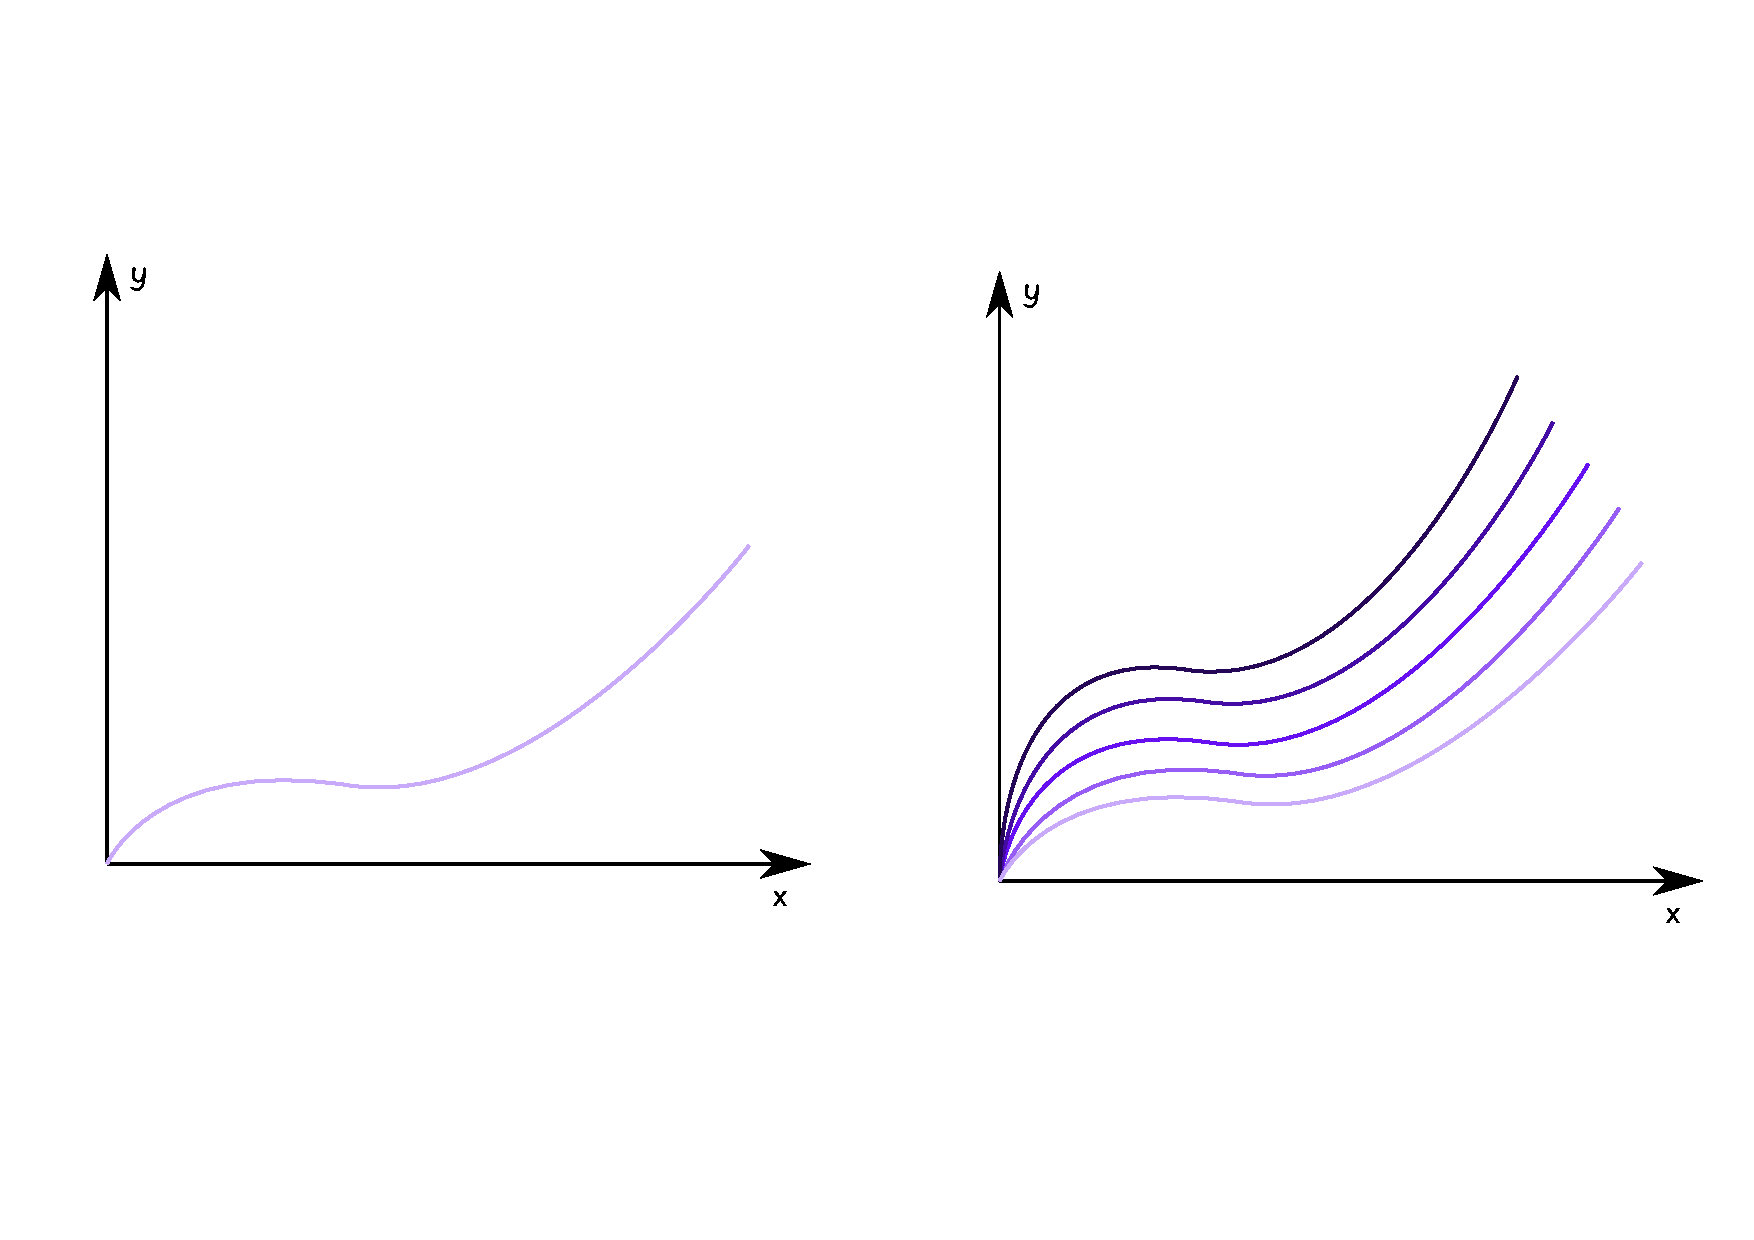
\includegraphics[width=0.75\textwidth]{singlevsmeta}
\end{frame}

\begin{frame}{But for why bother?}
\begin{minipage}{0.5\textwidth}
  \includegraphics<1>[width=\textwidth]{FE2}
  \includegraphics<2>[width=\textwidth]{FE2-ML}
\end{minipage}%
\begin{minipage}{0.5\textwidth}
  \begin{itemize}
    \item<1> Multi-scale composite modeling
    \item<1> Computational homogenization (nested FEA)
    \item<1> Computational expense is enormous

    \item<1-2>\dotfill

    \item<2> Currently: $\mathcal{M}(\mathbf{F}^\Omega,\cdot,\cdot)$
    \item<2> Computationally a material: $\mathbf{F}^\Omega\mapsto\mathbf{P}^\Omega$
    \item<2> Why not exploit the similarities?
  \end{itemize}
\end{minipage}
\end{frame}

\begin{frame}{For Example}
\begin{minipage}{0.5\textwidth}
  \includegraphics<1>[width=\textwidth]{example}
\end{minipage}%
\begin{minipage}{0.5\textwidth}
  \begin{itemize}
    \item<1> Focus on: $\mathcal{M}(\mathbf{F}^\Omega)$
    \item<1> Treat other descriptors as different tasks
  \end{itemize}
\end{minipage}
\end{frame}

\section{MAML vs Biased Ridge}
\begin{frame}{How to solve this problem?}
  \begin{itemize}
      \item Pool of methods and algorithms!
      \item One really famous and one promising but "overlooked" method!
  \end{itemize}
\end{frame}


\begin{frame}{MAML\cite{Finn2017}}
\begin{minipage}{0.5\textwidth}
  \includegraphics<1>[width=\textwidth]{maml}
\end{minipage}%
\begin{minipage}{0.5\textwidth}
  \begin{itemize}
    \item<1> Sample Tasks 
    \item<1> Sample training experiences from that tasks
    \item<1> Check the possible loses 
    \item<1> Take average step
  \end{itemize}
\end{minipage}
\centering
  \only<1> {For a model $\mathcal{M}$ parametrized by $(\mathbf{w})$}
\end{frame}

\begin{frame}{MAML\cite{Finn2017}}
  \begin{minipage}{0.5\textwidth}
    \includegraphics<1>[width=\textwidth]{maml_linear}
  \end{minipage}%
  \begin{minipage}{0.5\textwidth}
    \includegraphics<1>[width=\textwidth]{maml_nonlinear}
  \end{minipage}
\end{frame}

\begin{frame}{Biased Ridge\cite{Denevi2018a}}
\begin{minipage}{0.5\textwidth}
  \includegraphics<1>[width=0.95\textwidth]{ridge}
\end{minipage}%
\begin{minipage}{0.5\textwidth}
  \begin{itemize}
    \item<1> Sample Tasks 
    \item<1> Sample training experiences from that tasks
    \item<1> adjust the bias
  \end{itemize}
\end{minipage}
\centering
  \only<1>{ For a model $\mathcal{M}$ parametrized by $(\mathbf{w})$ minimize $\mathcal{L}+\lambda||\mathbf{w}-\mathbf{h}||^2_2$}

  \only<2>{ Kernel version: minimize $\mathcal{L}+\lambda||\mathcal{M}||^2_{\mathcal{H}_k}$}

\end{frame}

\section{Some Results/Conclusions}
\begin{frame}{Problem Setting-1}
  \begin{minipage}{0.5\textwidth}
    \color{Pink} Linear Problem \color{Black}
    \begin{itemize}
      \item<1> $ \mathbf{a} \in \mathbb{R}^d \to p_\mathcal{T} \sim \mathcal{N}(m\mathbf{1},c\mathbf{I})$
      \item<1>$ \mathbf{x} \in \mathbb{R}^d \to p_\mathbf{x} \sim \mathcal{N}(\mathbf{0},k\mathbf{1})$
      \item<1>$ \varepsilon \sim \mathcal{N}(0,\sigma^2)$
      \item<1>$ y = \mathbf{a}^\text{T}\mathbf{x} + \varepsilon \quad \in \mathbb{R}$
      \item<1>$ \mathcal{Z}:= ((x_i,y_i))_{i=1}^N$
      \item<1>$ \hat{\mathcal{M}} \to $ an estimator trained with $\mathcal{Z}$
    \end{itemize}
  \end{minipage}%
  \begin{minipage}{0.5\textwidth}
    \includegraphics<1>[width=0.9\textwidth]{lintask}
  \end{minipage}

\dotfill

  \color{Pink} Expected Error for an estimator: \color{Black}
  \centering
  $ \mathcal{E}:=\int \int \int (\hat{\mathcal{M}}-y)^2p(x,y)dxdyp_\mathcal{Z}d\mathcal{Z}p_\mathcal{T}d\mathcal{T}$
\end{frame}

\begin{frame}{Most Interesting Results}
  \centering
  \only<1>{
  Limit the number of gradient steps for adaptation to 1 and other parameters regarding the problem is defaulted to 1 as well.
  }

  \begin{minipage}{0.5\textwidth}
    \centering
    \includegraphics<1>[width=0.8\textwidth]{c_1_1}

    \only<1>{N=1}
  \end{minipage}%
  \begin{minipage}{0.5\textwidth}
    \centering
    \includegraphics<1>[width=0.8\textwidth]{c_1_10}

    \only<1>{N=10}
  \end{minipage}

  \only<2>{


    \color{Pink} Only consider the $c=[0,1]$ \color{Black}
  \begin{tabular}{c|c|c|c|c|c|c|c|c|c|c|c|}
    \cline{2-11}
     & \multicolumn{10}{|c|}{number of gradient steps}\\
    \cline{2-11}
     & 1 & 2 & 3 & 4 & 5 & 6 & 7 & 8 & 9 & 10\\
    \hline
    \multicolumn{1}{|c|}{MAML} & 1.21& \textbf{1.19} & 1.20& 1.21& 1.23& 1.24& 1.27& 1.33& 1.46& 1.75\\
    \hline
  \end{tabular}

  }
\end{frame}


\begin{frame}{Conclusions}
  \begin{minipage}{0.5\textwidth}
    \begin{itemize}
      \item<1> Benefit of MAML only for $p_\mathcal{T}$ with small variance...
      \item<2> Number of gradient steps taken is a clear regularizing effect...
      \item<2> Not, a huge gain though???
    \end{itemize}
  \end{minipage}%
  \begin{minipage}{0.5\textwidth}
    \includegraphics<1>[width=\textwidth]{task_variance}
  \end{minipage}
\end{frame}


\section{What is next?}
\begin{frame}{Method Development}
  \begin{itemize}
    \item Can we include additional bias for the functional norm in RKHS?
    \item Latent Variable Models for detecting underlying descriptors automatically?
  \end{itemize}
\end{frame}

\begin{frame}{Application}
  \begin{itemize}
    \item Bit by bit start using real-data for experimentation!
  \end{itemize}
\end{frame}

\begin{frame}
  \centering
  \color{Pink} Thanks!
\end{frame}

\section{Additional}
\begin{frame}{Problem Setting-2}
  \begin{minipage}{0.5\textwidth}
    \includegraphics<1>[width=0.9\textwidth]{nonlintask}
  \end{minipage}%
  \begin{minipage}{0.5\textwidth}
     \color{Pink} Nonlinear Problem \color{Black}
    \begin{itemize}
      \item<1> $ \mathbf{a} \in \mathbb{R}^d \to p_\mathbf{a} \sim \mathcal{N}(\mathbf{1},c_1\mathbf{I})$
      \item<1> $ \boldsymbol{\phi} \in \mathbb{R}^d \to p_{\boldsymbol{\phi}} \sim \mathcal{N}(\mathbf{0},c_2\mathbf{I})$
      \item<1> $ \mathbf{x} \in \mathbb{R}^d \to p_x \sim \mathcal{N}(\mathbf{0},k\mathbf{1})$
      \item<1> $ \varepsilon \sim \mathcal{N}(0,\sigma^2)$
      \item<1> $ y = \mathbf{a}^\text{T}\text{sin}(\mathbf{x}+\phi) + \varepsilon \quad \in \mathbb{R}$
      \item<1> $ \mathcal{Z}:= ((x_i,y_i))_{i=1}^N$
      \item<1> $ \hat{\mathcal{M}} \to $ an estimator trained with $N$ training points
    \end{itemize}
  \end{minipage}

\dotfill

  \color{Pink} Expected Error for an estimator: \color{Black}
  \centering
  $ \mathcal{E}:=\int \int \int (\hat{\mathcal{M}}-y)^2p(x,y)dxdyp_\mathcal{Z}d\mathcal{Z}p_\mathcal{T}d\mathcal{T}$
\end{frame}

\begin{frame}{Most Interesting Results}
  Every other parameter is defaulted to 1, and the adaptation steps used is 5.
  \begin{minipage}{0.33\textwidth}
    \centering
    \includegraphics<1>[width=\textwidth]{c2_1_1}
    N=1
  \end{minipage}%
  \begin{minipage}{0.33\textwidth}
    \centering
    \includegraphics<1>[width=\textwidth]{c2_1_10}
    N=10
  \end{minipage}%
  \begin{minipage}{0.33\textwidth}
    \centering
    \includegraphics<1>[width=\textwidth]{c2_1_50}
    N=50
  \end{minipage}%
\end{frame}


\end{document}
